% Created 2018-06-24 Dom 10:23
\documentclass[presentation]{beamer}
\usepackage[utf8]{inputenc}
\usepackage[T1]{fontenc}
\usepackage{fixltx2e}
\usepackage{graphicx}
\usepackage{grffile}
\usepackage{longtable}
\usepackage{wrapfig}
\usepackage{rotating}
\usepackage[normalem]{ulem}
\usepackage{amsmath}
\usepackage{textcomp}
\usepackage{amssymb}
\usepackage{capt-of}
\usepackage{hyperref}
\usetheme{default}
\author{Rafael G. Nagel}
\date{2018-06-22}
\title{Minimum Spanning Tree Algorithm (MST)}
\hypersetup{
 pdfauthor={Rafael G. Nagel},
 pdftitle={Minimum Spanning Tree Algorithm (MST)},
 pdfkeywords={},
 pdfsubject={},
 pdfcreator={Emacs 26.1 (Org mode 8.3.3)}, 
 pdflang={Pt-Br}}
\begin{document}

\maketitle
\begin{frame}{Outline}
\setcounter{tocdepth}{2}
\tableofcontents
\end{frame}



\section{Introduction}
\label{sec:orgheadline4}
\begin{frame}[label={sec:orgheadline1}]{Applications \footnote{\url{https://www.geeksforgeeks.org/applications-of-minimum-spanning-tree/}} and Problem}
\begin{itemize}
\item Usually relates to optimizations in \alert{network design}
\begin{itemize}
\item telephone
\item electrical
\item hydraulic
\item TV cable
\item road
\end{itemize}
\item Also indirect applications
\begin{itemize}
\item learning salient features for real-time face verification
\item max bottleneck paths
\end{itemize}
\end{itemize}
\end{frame}
\begin{frame}[fragile,label={sec:orgheadline2}]{Conditions}
 \begin{itemize}
\item graph G with \emph{positive} edge weights
\item \emph{undirected} edges
\item find a \alert{min weight} set of \emph{edges} that connects \alert{all} of the \emph{vertices}
\item number of \emph{edges} we want:
\begin{center}
\texttt{edges = number of vertices - 1}
\end{center}
\end{itemize}
\end{frame}

\begin{frame}[label={sec:orgheadline3}]{Few algorithms that implement MST \footnote{\url{https://www.ics.uci.edu/~eppstein/161/960206.html}}}
\begin{enumerate}
\item Kruskal's algorithm
\item Prim's algorithm
\item Boruvka's algorithm
\end{enumerate}

\rule{\linewidth}{0.5pt}
\begin{itemize}
\item Why did Kruskal?
\begin{itemize}
\item easier to code and understand
\end{itemize}
\end{itemize}
\end{frame}
\section{Algorithm explanation (Kruskal)}
\label{sec:orgheadline16}
\begin{frame}[fragile,label={sec:orgheadline5}]{Overview}
 \begin{enumerate}
\item order \emph{edges} by weight (ascendant)
\item pick edge and check if it forms a cycle with the spanning tree
\begin{itemize}
\item if cycle formed then discard edge
\item else include edge
\end{itemize}
\item repeat 2) until \texttt{e = v - 1}
\end{enumerate}
\end{frame}
\begin{frame}[label={sec:orgheadline6}]{How to check if graph has cycle?}
\begin{itemize}
\item Union-find\footnote{\url{https://www.geeksforgeeks.org/union-find/}} algorithm
\begin{itemize}
\item temporary vector to save parent of vertices being inserted
\end{itemize}
\end{itemize}

\begin{center}
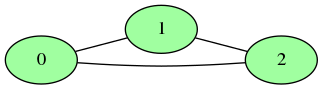
\includegraphics[width=0.5\textwidth]{images/union-find-example.png}

\begin{center}
\begin{tabular}{rrr}
0 & 1 & 2\\
-1 & -1 & -1\\
\end{tabular}
\end{center}

\begin{center}
\begin{tabular}{rrr}
\alert{0} & \alert{1} & 2\\
1 & -1 & -1\\
\end{tabular}
\end{center}

\begin{center}
\begin{tabular}{rrr}
0 & \alert{1} & \alert{2}\\
1 & 2 & -1\\
\end{tabular}
\end{center}
\end{center}
\end{frame}

\begin{frame}[label={sec:orgheadline7}]{Step by step with example\footnote{\url{https://www.geeksforgeeks.org/greedy-algorithms-set-2-kruskals-minimum-spanning-tree-mst/}}}
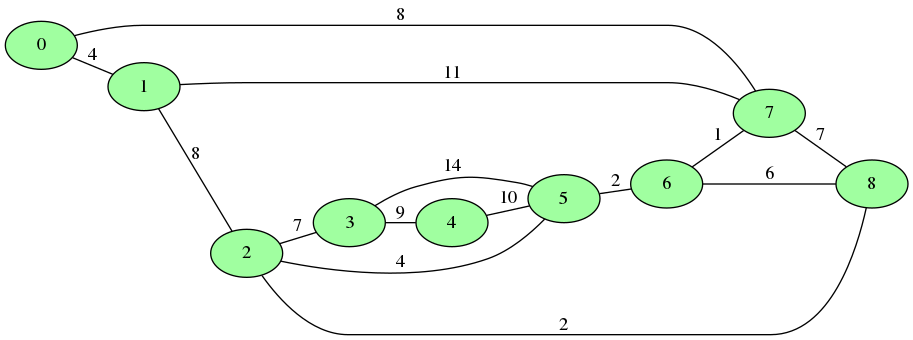
\includegraphics[width=1\textwidth]{images/example-1.png}
\end{frame}

\begin{frame}[label={sec:orgheadline8}]{Graph sorted by edges}
\begin{center}
\begin{tabular}{rrr}
weight & src & dst\\
\hline
1 & 7 & 6\\
2 & 8 & 2\\
2 & 6 & 5\\
4 & 0 & 1\\
4 & 2 & 5\\
6 & 8 & 6\\
7 & 2 & 3\\
7 & 7 & 8\\
8 & 0 & 7\\
8 & 1 & 2\\
9 & 3 & 4\\
10 & 5 & 4\\
11 & 1 & 7\\
14 & 3 & 5\\
\end{tabular}
\end{center}
\end{frame}

\begin{frame}[label={sec:orgheadline9}]{pick edges from sorted and try to include each one}
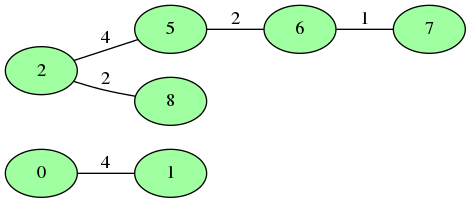
\includegraphics[width=0.7\textwidth]{images/example-1-step-1.png}

\ldots{} no cycles so far.

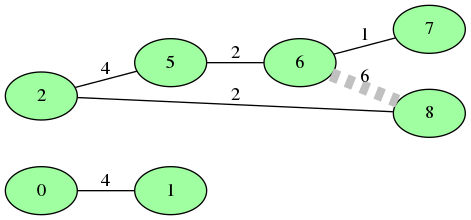
\includegraphics[width=0.6\textwidth]{images/example-1-step-3.png}

\ldots{} including 8-6 produces a cycle. Do not include it.
\end{frame}

\begin{frame}[fragile,label={sec:orgheadline10}]{repeat until: \texttt{edges = vertices - 1}}
 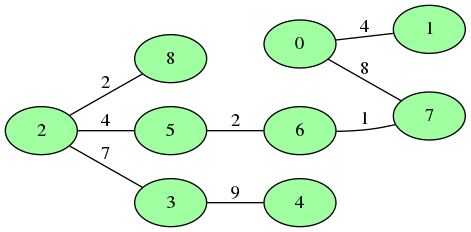
\includegraphics[width=.9\linewidth]{images/example-1-step-4.png}
\end{frame}

\begin{frame}[label={sec:orgheadline11}]{Complexity}
\begin{block}{summing up:}
\begin{enumerate}
\item sort graph ascendant (qsort \(\to\) O(nlogn))
\item apply MST (Kruskal) algorithm
\begin{enumerate}
\item for \emph{each edge} in sorted list:
\begin{enumerate}
\item include it in MST graph
\item check if \emph{formed cycle}; if so remove it
\end{enumerate}
(find-union algorithm)
\end{enumerate}
\end{enumerate}
\end{block}
\begin{block}{Kruskal complexity}
\begin{itemize}
\item The find-union is O(n) in the \emph{present work}
\begin{itemize}
\item we could improve it to O(logn) using \emph{union by Rank or Height}\footnote{\url{https://www.geeksforgeeks.org/union-find/}}
\end{itemize}
\end{itemize}
\end{block}
\end{frame}
\begin{frame}[fragile,label={sec:orgheadline12}]{Complexity}
 \begin{block}{Consider the worst case}
\begin{itemize}
\item Everytime we add a new vertice in a graph, we can have:

\begin{center}
\texttt{edges + = number of vertices - 1}. 
\end{center}

\item Thus, number of edges in the worst case is:

\begin{center}
edges = \(v^{2}\) \\
when edges \(\to\) \(\infty\)
\end{center}
\end{itemize}
\end{block}


\begin{block}{This implementation:}
\begin{center}

\(O(e \times \log{e}) + O(e  \times O(v)) \\
    O(e \times \log{e} + v^{2} \times v) \\
    O(e \times \log{v} + v^{3}) \\\)
\end{center}
\end{block}
\end{frame}
\begin{frame}[fragile,label={sec:orgheadline13}]{Complexity}
 \begin{block}{Implementation with: \texttt{union-find = O(logn)}}
\begin{center}

\(O(e \times \log{e}) + O(e \times \log{v}) \\
    e = v^{2} \to \log{e} = \log{v^{2}} = 2 \times \log{v} \approx \log{v} \\
    \therefore \\
    O(e \times (\log{v} + \log{v})) = O( e \times 2 \times \log{v} ) \\
    \therefore \\
    O(e \times \log{v}) \\\)
\end{center}
\end{block}
\end{frame}

\begin{frame}[label={sec:orgheadline14}]{Code}
\begin{block}{Structs}
\begin{itemize}
\item grafo
\item vertice
\item lista
\item nó
\end{itemize}
\end{block}

\begin{block}{New functions}
\begin{itemize}
\item hasCycle()
\item union()
\item find()
\end{itemize}
\end{block}
\end{frame}

\begin{frame}[label={sec:orgheadline15}]{Conclusion}
\begin{itemize}
\item Instead of creating new \emph{structs} or \emph{files}, I add \emph{members} to structs and add new \emph{functions} to files
\end{itemize}
\begin{block}{How to avoid checking \alert{double vertice addition} without \alert{O(n)}?}
\begin{itemize}
\item With this issue, the complexity has one more \emph{v} factor:
\begin{center}
\(O(e \times \log{v} + v^{4})\)
\end{center}
\end{itemize}
\end{block}

\begin{block}{Kruskal algorithm is \emph{much easier} to implement than other}
\begin{itemize}
\item Tradeoffs: Complexity vs. Time of coding
\end{itemize}
\end{block}
\end{frame}
\end{document}
